%%%%%%%%%%%%%%%%%%%%%%%%%%%%%%%%%%%%%%%%%%%%%%%%%%%%%%%%%%%%%%%%%%%%%%%%%%%%%%%%%%%%%%%%%%%%%%%%%%%%
% Project proposal report
% Authors: Michael Galliers and James Miller
% Course: CSC 440
%%%%%%%%%%%%%%%%%%%%%%%%%%%%%%%%%%%%%%%%%%%%%%%%%%%%%%%%%%%%%%%%%%%%%%%%%%%%%%%%%%%%%%%%%%%%%%%%%%%%

\documentclass[12pt]{article}
\usepackage[utf8]{inputenc}
\usepackage{graphicx}
\usepackage{float}

% Document configuration

% Section numbering
\renewcommand \thesection{\Roman{section}}
\renewcommand \thesubsection{\arabic{section}.\arabic{subsection}}
% Do paragraph indenting after section tags
\usepackage{indentfirst}


\usepackage[usenames, dvipsnames]{color}
\author{Michael Galliers and James Miller}
\title{CSC 440 - Project Proposal}
\date{August 27, 2019}


\begin{document}

\begin{titlepage}
\maketitle
\end{titlepage}

\newpage
    \tableofcontents
\newpage

\section{Project Overview}
For our team and individual projects in CSC 440 this Fall semester, we have decided to make a grade
tracking web application. Our proposed codename for the project is \textbf{Griefer} (actual project
name TBD).

\subsection{Problems and Needs}
The idea for this project arose from personal experience, not being able to effectively manage
grades from various courses on BlackBoard. This can be due to professors not using BlackBoard to
distribute grades or the inability of BlackBoard to correctly aggregate student grades because of
an odd grading policy. This makes it difficult for students to track how well they are doing in a
course overall. As a result, students can be more or less likely to study hard for assignments,
since they believe they are doing worse or better in the course than they potentially are.

For those who decide to manage their grades themselves with pen and paper, they are able to gain
further insight into their performance in courses, but are limited by the amount of time it takes to
manage and compute statistics about their grades. As a student, there should be a simple way to
manage and visualize grades, without the need to do calculations by hand.

\subsection{System Requirements}
As a solution to these problems, we propose a web-based software application. This application shall
include, but not be limited to, the following requirements:

\begin{itemize}
    \item Allow a student to create, retrieve, update and delete semesters.
    \item Allow a student to create, retrieve, update and delete courses in each semester.
    \item Allow a student to create, retrieve, update and delete categories in each course. (e.g.
    homework, tests, etc.).
    \item Allow a student to create, retrieve, update and delete grade entries in each category.
    \item Allow different grading strategies to be used for each course, i.e. total point based vs.
    weight based.
    \item Account for additional grading requirements in a course (e.g. to get an 'A' you need at
    least a 90\% overall and at least 80\% in each category).
    \item Include visualizations/summaries for how well a student is doing in a course, category or
    the semester overall.
    \item Provide feedback to a student on his/her performance in a course and improvements that
    can be made.
    \item Include a "What If" feature, allowing a student to see how a score on a particular
    assignment would effect his/her overall grade.
\end{itemize}

\section{Goals}
\subsection{Project}
In building this project, we intend to use a modern software development stack. As a result, our
team will strive to gain knowledge in the following technologies/principals:

\begin{itemize}
    \item React.js and Javascript for the frontend
    \item Python for the backend
    \item JetBrains development IDEs
    \item Continuous Integration and Continuous Deployment (CI/CD, with automated software testing)
    \item Git source control
    \item Container-based application deployment
\end{itemize}

\subsection{Product}
The key goal of the product is to make the lives of students easier. Students should be able to
quickly see their performance in a course without having to do manual calculations/approximations.
Our advantage in developing this tool is that we, as developers, are also part of the target
audience: students. As a result, our goal is to quickly elicit the requirements and design the
product to fit its needs using our knowledge of the problems.

\section{System Workflow}
\begin{figure}[H]
  \centering
  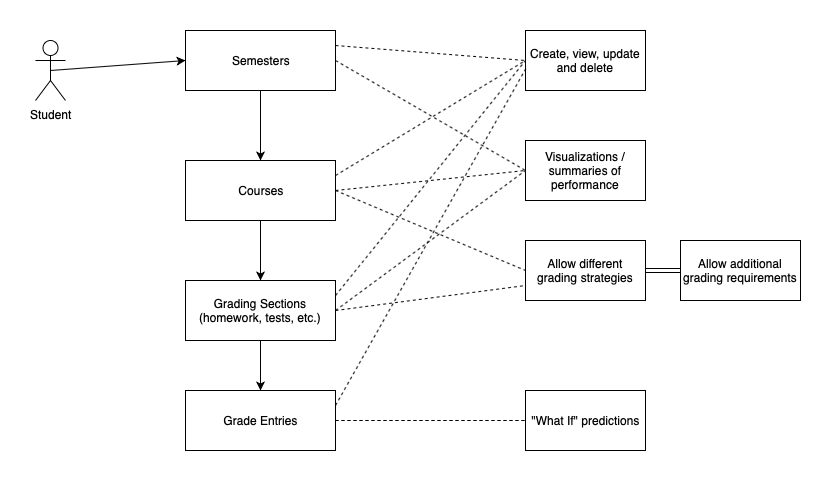
\includegraphics[width=\linewidth]{resources/workflow_diagram.png}
  \caption{Workflow Diagram - A high level overview of the system}
\end{figure}

\section{Required Resources}
\subsection{Hardware}
For deployment of our application, we are planning on utilizing cloud based computing hardware for
running the backend, serving the frontend, and managing the database. Our final decision on a
specific cloud provider is subject to change, but the hosting service \textit{Digital Ocean} is a
possibility. It offers reasonable pricing and should allow us to get the application deployed in a
short amount of time.

\subsection{Software}
This app will be designed in two subsystems: the web browser-based frontend and server-side backend.
The frontend shall communicate with the backend using a REST API with web browser requests (AJAX) to
send/receive information. In building this project, we plan on using a modern software development
stack. This includes the following software/technologies:

\begin{itemize}
    \item React.js and Javascript for the frontend
    \item Python for the backend
    \item JetBrains development IDEs
    \item Git with GitHub for source control
    \item GitHub-integrated CI service for automatic building, testing and deploying
    \item Docker/Kubernetes for scalable containerized deployments
    \item PostgreSQL relational database
\end{itemize}

\section{Dictionary}
\begin{itemize}
    \item \textbf{Semester}: A single semester of education consisting of courses. Each semester can
    be associated with a different educational institution; consistency is not required.
    \item \textbf{Course}: Any educational course/class occurring within a particular semester.
    \item \textbf{Section}: An equally weighted or logically grouped collection of material within a
    particular course (e.g. Homework, Tests, etc.).
    \item \textbf{Grade Entry}: A graded piece of material associated with a particular section 
    (e.g. Homework 2, Exam 1, etc.).
\end{itemize}

\end{document}
